\documentclass[a4paper]{article}

\usepackage[utf8]{inputenc}
\usepackage[top=3cm,bottom=3cm,left=2.5cm,right=2.5cm]{geometry}
\usepackage[T1]{fontenc}           % For symbols like tilde
\usepackage{hyperref}              % For \url{...}
\usepackage{amsthm}                % \proof environment
\usepackage{amssymb}               % Math symbols
\usepackage{amsmath}               % Various commands like \text{...}
\usepackage{mathtools}             % Maths
\usepackage[noend]{algpseudocode}  % Pseudocode printer
\usepackage{listings}              % Source code printer
\usepackage{framed}                % To frame the computational cost
\usepackage{qtree}                 % Draw simple binary trees
\usepackage{titlesec}              % Customize sections
\usepackage{biblatex}              % Bibliography
\usepackage{FiraSans}              % Font for the title
\usepackage{tikz}                  % Drawing
\usepackage{tikz-qtree}            % Drawing trees
\usetikzlibrary{matrix}
\addbibresource{bibliography.bib}

\DeclarePairedDelimiter\abs{\lvert}{\rvert}  % Define abs-like syntax
\DeclarePairedDelimiter\norm{\lVert}{\rVert}
\DeclareMathOperator*{\median}{median}       % Median operator with subscript support
\DeclareMathOperator*{\mprob}{\mathbb{P}}    % Probability with subscript support

\newcommand*{\E}[1]{\mathbb{E}\left[{#1}\right]}      % Define expected value
\newcommand*{\prob}[1]{\mprob\left[{#1}\right]}       % Define probability
\newcommand*{\probs}[2]{\mprob_{#1}\left[{#2}\right]} % Define probability with subscript
\newcommand{\sectionbreak}{\clearpage}                % Clear page before each section

\lstset{numbers=left} % Print line numbers in \begin{lstlisting}...

\title{\rule{12cm}{2pt} \vspace{5mm} \\ \Huge\firaoldstyle{Advanced Algorithms:\\ Problems and Solutions} \rule{12cm}{4pt}}
\author{\Large\firalight{Mattia Setzu} \and \Large \firalight{Giorgio Vinciguerra}}
\date{\firathin{2016}}

\begin{document}

  \maketitle
  \tableofcontents

  \section{Range updates}

Consider an array $C$ of $n$ integers, initially all equal to zero. We want to support the following operations:
\begin{itemize}
  \item $update(i, j, c)$, where $0 \leq i \leq j \leq n - 1$ and $c$ is an integer: it changes $C$ such that $C[k] := C[k] + c$ for every $i \leq k \leq j$.
  \item $query(i)$, where $0 \leq i \leq n - 1$: it returns the value of $C[i]$.
  \item $sum(i,j)$, where $0 \leq i \leq j \leq n - 1$: it returns $\sum_{k = 1}^j C[k]$.
\end{itemize}

Design a data structure that uses $O(n)$ space, takes $O(n \log n)$ construction time, and implements each operation above in $O(\log n)$ time. Note that $query(i) = sum(i, i)$ but it helps to reason.

[Hint: For the general case, use the segment tree seen in class, which uses $O(n \log n)$ space: prove that its space is actually $O(n)$ when it is employed for this problem.]

\vspace{0.5cm}
\paragraph{Solution.}
We use a segment binary tree $T_I$ over the interval $I = [0, n - 1]$, that is, a tree whose leaves are the points in $I$ and the parent of two nodes is the union of their interval. More formally, if $x.interval$ denotes the attribute $interval$ of the node $x$,
\begin{enumerate}
  \item $l.interval \cup r.interval = n.interval \iff n \text{ is the parent of $l$ and $r$}$;
  \item $\text{if $x$ and $y$ are leaves, then } x.interval \cap y.interval = \emptyset \wedge |x.interval|=|y.interval|=1$.
\end{enumerate}
For example, the segment tree for $I=[0,7]$ is the following:
\begin{center}
  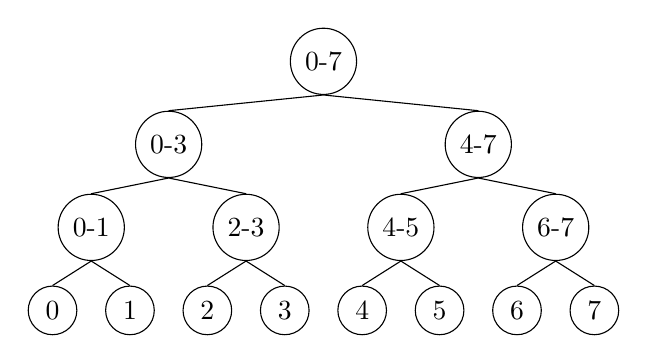
\begin{tikzpicture}[sibling distance=10pt]
    \tikzstyle{every node}=[circle,draw]
    \Tree [.0-7 [.0-3 [.0-1 [.0 ]  [.1 ] ] [.2-3 [.2 ] [.3 ] ] ] [.4-7 [.4-5 [.4 ] [.5 ] ] [.6-7 [.6 ] [.7 ] ] ] ]
  \end{tikzpicture}
\end{center}

We associate with each node $x$ of $T_I$ some attributes: $x.sum$, that stores $\sum_{i \in x.interval} C[i]$; and $x.lazy$, that stores a value that need to be propagated to each descendant of $x$. This means that $x.sum$ might not be accurate at a given time for any of the requested operation.  

\paragraph{Range operations.} In both operations we traverse the tree recursively starting from the root and, at \emph{each} recursive step on any internal node $x$, if $x.lazy \neq 0$: we set $x.sum \gets x.sum + |x.interval| \times x.lazy$, we propagate the lazy information to $x$'s children $x.left.lazy \gets x.lazy$, $x.right.lazy \gets x.lazy$ and, finally, we reset the information $x.lazy \gets 0$. Afterwards, if the operation is 
\begin{itemize}
  \item $sum(i,j)$, we do the following:
  \begin{enumerate}
    \item if $x.interval \cap [i,j] = \emptyset$, we return 0;
    \item if $x.interval \subseteq [i,j]$, we return $x.sum$;
    \item otherwise we repeat the procedure $sum(i,j)$ on $x.left$ and $x.right$, returning the sum of these calls.
  \end{enumerate}

  \item $update(i,j,c)$, we do the following:
  \begin{enumerate}
    \item if $x.interval \cap [i,j] = \emptyset$, we stop the recursion on this subtree;
    \item if $x.interval \subseteq [i,j]$, we update $x.sum \gets |x.interval| \times c$, and $x.left.lazy \gets x.left.lazy + c$, $x.right.lazy \gets x.right.lazy + c$
    \item otherwise we repeat the procedure $update(i,j,c)$ on $x.left$ and $x.right$.
  \end{enumerate} 
\end{itemize}
The space occupied by $T_I$ is $\sum_{i=0}^{\log_2 n} n/2^{-i}=2n-1$.
  \section{Depth of a node in a random search tree}

A random search tree for a set S can be defined as follows: if $S$ is empty, then
the null tree is a random search tree; otherwise, choose uniformly at random a key
$k$ as root, and the random search trees on $L = \{x \in S : x < k\}$ and $R = \{x \in S :
x > k\}$ become, respectively, the left and right subtree of the root $k$.
Consider the randomized QuickSort discussed in class and analyzed with indicator
variables \href{http://didawiki.cli.di.unipi.it/lib/exe/fetch.php/magistraleinformatica/alg2/algo2_13/randqs.pdf}{CLRS 7.3},
and observe that the random selection of the pivots follows the above process,
with indicator variables, prove that:
\begin{enumerate}
  \item the expected depth of a node (i.e.\ the random variable representing the distance of the node from the root) is nearly $2 \ln n$;
  \item the expected size of its subtree is nearly $2 \ln n$ too, observing that it is a simple variation of the previous analysis;
  \item the that the probability that the depth of a node exceeds $c2 \ln n$ is small for any given constant $c > 1$.
\end{enumerate}

\subsection{Proof with indicator variable}

\paragraph{Prove that the expected depth of a node is nearly $2 \ln n$.}

\begin{proof}
  Let $z_m$ the $m$th smallest element in $S$ and $$X_{ij}=
  \left\{
    \begin{array}{ll}
      1 & \mbox{if $z_j$ is an ancestor of $z_i$ in the random search tree} \\
      0 & \mbox{otherwise}
    \end{array}
  \right.$$
  The depth of the node $i$ in the tree is given by the number of its ancestors:
  \begin{equation}
    X=\sum_{\substack{j=1 \\ j\ne i}}^n X_{ij}
    \label{equation:node-depth}
  \end{equation}

  Note that the depth of a node is also equal to the number of comparison it's
  involved in (in other words, the number of times it became the left or the
  right child of a randomly chosen pivot).

  Once a pivot $k$ is chosen from $S$, $S$ is partitioned in two subsets $L$ and
  $R$. The elements in the set $L$ will not be compared with the elements in $R$
  at any subsequent time. The event $E_1=$ ``$z_j$ is an ancestor of $z_i$ in the
  random search tree'' occurs if $z_j$ and $z_i$ belong to the same partition
  \emph{and} $z_j$ was chosen as pivot before $z_i$. The probability that $E_1$
  occurs, since it is the intersection of two events, can be upper bounded by:
  $$\text{Pr}\{ z_j \text{ was chosen as pivot before } z_i
  \}=\frac{1}{\text{size of the partition}}\leq\frac{1}{|j-i|+1}$$ because
  pivots are chosen randomly and independently, and because the partition that
  contains both $z_j$ and $z_i$ must contain \emph{at least} the $|j-i|+1$
  numbers between $z_j$ and $z_i$.

  Taking expectations of both sides of~\eqref{equation:node-depth}, and then
  using linearity of expectation, we have:
  \begin{align*}
    \E{X} & = \sum_{\substack{j=1\\ j\ne i}}^n \E{X_{ij}} \\
    & = \sum_{\substack{j=1\\ j\ne i}}^n \text{Pr}\{ z_j \text{ is an ancestor
      of } z_i \text{ in the random search tree} \} \\
    & \le \sum_{\substack{j=1\\ j\ne i}}^n \frac{1}{|j-i|} \\
    & = \sum_{j=1}^{i-1} \frac{1}{i-j} + \sum_{j=i+1}^{n} \frac{1}{j-i}
  \end{align*}
  With the change of variables $l=i-j$ and $m=j-i$:
  \begin{equation*}
    = \sum_{l=1}^{i-1} \frac{1}{l} + \sum_{m=1}^{n} \frac{1}{m} \approx 2\ln n
  \end{equation*}

\end{proof}

\paragraph{Prove that the expected size of its subtree is nearly $2 \ln n$ too,
observing that it is a simple variation of the previous analysis.}

\begin{proof}
  The size of the subtree of a randomly chosen pivot of $z_j\in S$ is given by
  the number of it's descendants. Since~\eqref{equation:node-depth} is the
  number of ancestors of a node $z_i$, we can find the number of descendants of
  $z_j$ by changing the summation from $j=1,\dotsc,n$ to $i=1,\dotsc,n$.
\end{proof}

\paragraph{Prove that the that the probability that the depth of a node exceeds $c2 \ln n$ is small for any given constant $c > 1$.}

\begin{proof}
  We apply the Theorem \ref{theorem:chernoff} below with $(1+\delta)=c$ and $\mu=2 \ln n$:
  $$\prob{X>2c\ln n}<\left(\frac{e^{c-1}}{c^c}\right)^{2 \ln n}$$
  Since $\lim_{n\to+\infty}a^n=0$ with $0<a<1$, and $\lim_{n\to+\infty}2\ln n= +\infty$, we have to prove that, for any $c>1$
  $$0<\frac{e^{c-1}}{c^c}<1$$
  The first inequality is simple to verify, for the latter observe that
  $$\frac{e^{c-1}}{c^c}<1 \iff e^{c-1}<c^c \iff c-1 < c\ln c \iff c(1-\ln c)<1.$$
\end{proof}

\newtheorem{thm}{Theorem}
\begin{thm}[Chernoff Bound]\label{theorem:chernoff}
  Let $X_1, \dots, X_n$ be independent Poisson trials such that, for $1 \leq i \leq n$, $\prob{X_i=1}=p_i$, where $0 < p_i < 1$. Then, for $X=\sum_{i=1}^n X_i$, $\mu=\E{X}=\sum_{i=1}^n p_i$ and any $\delta>0$,
	$$\prob{X>(1+\delta )\mu}<\left({\frac {e^{\delta }}{(1+\delta )^{(1+\delta )}}}\right)^\mu.$$
\end{thm}
  \section{Karp-Rabin fingerprinting on strings}

Given a string $S: |S| = n$, and two positions $0 \leq i < j \leq (n - 1)$,
the longest common extension $lceS(i, j)$ is the length of the maximal run of matching
characters from those positions, namely: if $S[i] 6= S[j]$ then $lceS(i, j) = 0$;
otherwise, $lceS(i, j) = \max{l \geq 1 : S[i ... i + l - 1] = S[j ... j + i - 1]}$.
For example, if S = abracadabra, then $lceS(1, 2) = 0$, $lceS(0, 3) = 1$, and
$lceS(0, 7) = 4$.
Given S in advance for preprocessing, build a data structure for S based
on the Karp-Rabin fingerprinting, in $O(n \ln(n)$) time, so that it supports subsequent
    \begin{itemize}
    \item $lceS(i, j)$: it computes the longest common extension at positions i
    \item $equals (i, j, c)$: it checks if $S[i ... i + ` - 1] = S[j ... j + ` - 1]$ in constant time.
    \end{itemize}
Analyze the cost and the error probability.
The space occupied by the data structure can be $O(n \log(n))$ but it is possible
to use $O(n)$ space.
[Note: in this exercise, a onetime preprocessing is performed, and then many online
queries are to be answered on the fly.]

\subsection{Solution 1: Cumulative shift}
\subsubsection{Construction}

In order to save computational cycles on checks over ranges we use a similar structure
to the one in the range updates: we compute the hashing on the first character in $O(1)$
time, then roll the hash through the $n - 1$ remaining characters through $n O(1)$
operations.
We call $H$ this array; we also denote $h_k$ as the function $c a^{i}$ computating
the Rabin-Karph hash of a string $s$.
The reader shall now see that $\exists h^{-1}(s)$: that is, $h$ is invertible in $O(1)$.
The entries $h[i] = \sum_{i \in [0, n - 1]}(h(i))$ have cumulative hash and the following
properties hold:
    \begin{itemize}
    \item $h[s[i]] = (h[i] - h[i - 1]) / a^{-1}, a^{-1} = a^{1}$
    \item $h[i..j] - h[k..l] = (h[l] - h[k - 1]) / a^{-1} -
            (h[j] - h[i - 1]) / a^{-1}, a^{-1} = \textrm{modular inverse}$
    \end{itemize}

\subsubsection{equals(i, j, l)}

\textsc{equals} works on cumulative hashes, subtracting them and scaling them
accordingly, as our $rabin$ function multiplies by an $a^{i}$ costant.

\begin{algorithmic}[1]
  \Function{equals}{$i$, $j$, $length$}:
    \State $h_i = h[i + length] - h[i - 1]$\;
    \State $h_j = h[j + length] - h[j - 1]$\;

    \State $h^{i} = h_i / inv(a, i, l)$\;
    \State $h^{j} = h_j / inv(a, j, l)$\;

    \Return{$h^{i} - h^{j} == 0$}\;
    \EndFunction

    \Function{inv}{$h$, $k$, $l$}:
    \Return $h^{k - l}$
    \EndFunction
\end{algorithmic}

\subsubsection{lce(i, j)}

\textsc{lce} works on cumulative hashes, checks the equality on the middle element
of the strings and runs recursively on the half with different hashing.
We define \textsc{lce} as an auxiliary function

\begin{algorithmic}[1]
  \Function{lce}{$i$, $j$, $l$}:
    \State eq = \Call{equals}{$i$, $j$}\;

    \If{eq}
        \Return{$l$}
    \ElsIf{$\neg$ \Call{equals}{$(j - i) / 2$, $(n - j) / 2$, $l$}}
        \Return{\Call{equals}{$(j - i) / 2$, $(n - j) / 2$}}                            % First half
        \Else $(j - i) / 2 + $ \Return{\Call{equals}{$(j - i) / 2$, $(n - j) / 2$}}     % Second half
    \EndIf

    \State $h_i = h[i + length] - h[i - 1]$\;
    \State $h_j = h[j + length] - h[j - 1]$\;

    \State $h^{i} = h_i / inv(a, i, l)$\;
    \State $h^{j} = h_j / inv(a, j, l)$\;

    \Return{$h^{i} - h^{j} == 0$}\;
    \EndFunction

    \Function{inv}{$h$, $k$, $l$}:
    \Return $h^{k - l}$
    \EndFunction
\end{algorithmic}

  \section{Hashing sets}

Your company has a database $S \subseteq U$ of keys. For this database, it uses a hash function $h$ uniformly chosen at random from a universal family $\mathcal{H}$ (as seen in class); it also keeps a bit vector $B_S$ of $m$ entries, initialized to zeroes, which are then set $B_S[h(k)] = 1$ for every $k \in S$ (note that collisions may happen). Unfortunately, the database $S$ has been lost, thus only $B_S$ and $h$ are known, and the rest is no more accessible. Now, given $k \in U$, how can you establish if $k$ was in $S$ or not? What is the probability of error? [Note: you are not choosing $k$ and $S$ randomly as the they are both given... randomization here is in the choice of $h \in \mathcal{H}$ performed when building $B_S$.] Under the hypothesis that $m \geq c|S|$ for some $c > 1$, find the expected number of 1s in $B_S$ under a uniform choice at random of $h \in \mathcal{H}$.

\vspace{0.5cm}
\paragraph{Solution.}
Trivially for $B_s[h(k)] = 0$ we can answer \textsc{false} with $\prob{error} = 0$.
Let us analyse the opposite case, $B_s[h(k)] = 1$.
Let $i \in [0,m]$ be some index s.t. $B_s[i] = 1$, and let $cl_{S}(i)$ be the list of $k \in S: h(k) = 1$ for some set $S \in \displaystyle {\mathcal {P}}(S)$.
We can then denote the sets $cl_{U} := \{k_{U} : k_{U} \in U, h(k) = i\}, cl_{S} := \{k_{S} : k_{S} \in S, h(k) = i\}$; it is trivial to show that
    \begin{itemize}
    \label{6_cl_inclusion} \item $cl_{S} \subseteq cl_{U}$ as $S \in U$.
    \label{6_cl_length} \item $| cl_{S}(k) | \leq | cl_{U}(k) | \forall k \in U$ as $S \subseteq U$.
    \end{itemize}
Let us now try and estimate $|cl_{S}(k)|$: given $h$ is universal, we have an expected number of collisions of $\E{X_{k}} \approx \frac{1}{m} \forall k \in S$, that is
\begin{align*}
    \prob{h(k^{0}) = c} = \frac{1}{m}                               					\\
    \prob{h(k^{0}) = c, h(k^{1}) = c} = \left(\frac{1}{m}\right)^{2}                    \\
    \prob{h(k^{j}) = c, \dots, h(k^{j + i} = c)} = \left(\frac{1}{m}\right)^{j - i}    	\\
    \prob{h(k) = c, \forall k \in S} = \left(\frac{1}{m}\right)^{|S|}
\end{align*}
We can similarly compute the probability of not collision by simply replacing $\frac{1}{m}$ with $(1 - \frac{1}{m})$:
\begin{equation*}
  \prob{h(k) != c, \forall k \in S} = \left(1 - \frac{1}{m}\right)^{|S|}
\end{equation*}

Given our estimate of the collision list, we can now compute an estimate of the error probability: by~\ref{6_cl_inclusion}, we give an erroneous answer whenever $k \in cl_{U}(k), k \notin cl_{S}(k)$, that is we have a margin of error of $cl_{U}(k) \setminus cl_{S}(k)$ whose size is $|cl_{U}(k)| - |cl_{S}(k)|$.
Given the set of $k$ for which $h(k) = i$ the \emph{bad answers} are then
    \begin{equation}
    1 - \prob{\textrm{S hit the given cell}} = 1 - \left(1 - \frac{1}{m}\right)^{|S|}
    \end{equation}
We now provide a lower and upper bound for the said value.
The lower bound is given by the \emph{perfect hash} with no collisions: given
$e = $ number of $1$ in $B_s$, $e$ is the lowerbound.
Provided that  $m \geq c |S|$ for some $c > 1, |S| \leq \frac{m}{c}$:
    \begin{equation}
    \prob{\textrm{collision over i}} = \alpha_{S} = \frac{\frac{m}{c}}{m} = \frac{1}{c}
    \end{equation}
Therefore
    \begin{equation}
    e \leq 1 - \frac{1}{m^{|S|}} \leq \frac{1}{c}
    \end{equation}

\paragraph{Expected number of 1 in $B_{s}$.}
We define a random variable $X_{k}$:
    \begin{equation*}
    X_{k} = \begin{cases}
            1   & if B_{s}[k] = 1  \\
            0   & otherwise
            \end{cases}
    \end{equation*}
and one over the ones in $B_{s}$, $X$:
    \begin{equation}
        X = \sum_{k = 0}^{m - 1}X_k
    \end{equation}
We compute the relative expected value $\E{X}$:
    \begin{align*}
       \E{X} & = \E{\sum_{k = 0}^{m - 1}X_k} \\
       & = \sum_{k = 0}^{m - 1} \left( \prob{B_{s}[k] = 1} \right) \\
       & = \sum_{k = 0}^{m - 1} \left( \frac{\alpha}{m}\right) \leq \frac{m}{c}
   \end{align*}
where $\prob{B_{s}[k] = 1} = \frac{\alpha}{m}$ as $\alpha$ are the favourable cases
(i.e. the collisions for a generic bucket $B_s[i]$), and $m$ is the size of $B_s$.
  \include{5-uniform-hash-functions}
  \section{Deterministic data streaming}

Consider a stream of $n$ items, where items can appear more than once in the stream.
The problem is to find the most frequently appearing item in the stream (where ties
broken arbitrarily if more than one item satisfies the latter).
Suppose that only $k$ items can be stored, one item per memory cell, where the
available storage is $k + O(1)$ memory cells.
Show that the problem cannot be solved deterministically under the following rules:
the algorithm can allocate only $O(poly\log(n))$ bits for each of the $k$ items that
it can store (i.e. $O(\log^{c}(n))$ for any fixed costant $c$ > 0), and can read
the next item of the stream; you, the adversarty, have access to all the stream,
and the content of the $k$ items stored by the algorithm, and can decide what is
the next item that the algorithm reads (please note that you cannot change
past, namely, the items already read by the algorithm).
\\Hint: it is an adversarial argument based on the k items chosen by the
hypothetical determinist streaming algorithm, and the fact that there can be a
tie on $> k$ items till the last minute.

  \section{Special case of most frequent item in the stream}

Suppose to have a stream of $n$ items, so that one of them occurs $> \frac{n}{2}$
times in the stream.
Also, the main memory is limited to keeping just two items and their counters, plus
the knowledge of the value of $n$ beforehand.
Show how to find deterministically the most frequent item in this scenario.
\\ Hint: since the problem cannot be solved deterministically if the most
frequent item occurs $\leq \frac{n}{2}$ times, the fact that the frequency is
$> \frac{n}{2}$ should be exploited.

\vspace{0.5cm}
\paragraph{Solution.}
We'll use the notation of the previous section.
Before illustrating our solution we prove that the following hold:
    \begin{itemize}
    \label{frequence_dominance}\item \textbf{Given the $j^{1}$ element, $C(j^{1}) > C(j^{i}) \forall i \in S$.}
    \item Following the previous, $C(j^{i}) < C(j^{i}),  i > 1$ element.
    \item \textbf{There are at most $\frac{n}{2} - 1$ elements in S:} given that $j^{1}$
    appears at least $\frac{n}{2} + 1$ times, in the best case scenario every
    other $\frac{n}{2} - 1$ element is different, giving $\frac{n}{2} - 1$
    different elements.
    \label{sub-stream_dominance}~\item \textbf{$j^{1}$ has sub-stream dominance:}
    $\exists S' \subseteq S: j^{1} \textrm{ is the most frequent item} \in S'$:
    trivially, since it is the most frequent element, $S'$ is always a sub-stream
    dominant sub-stream.
    \end{itemize}

\paragraph{Recursive sub-streams} It is trivial to show that if we were to have
$\frac{n}{2}$ counters, $\Sigma^{\frac{n}{2}}_{i = 0, i \neq 1}(C(j^{i}) < C(j^{1})$
by~\ref{frequence_dominance}.
Though trivial, by combining it with~\ref{sub-stream_dominance} we can assert that
given $S' = S[0, \frac{n}{2}], S'' = S[\frac{n}{2}, n], k = \textrm{ number of elements } \in S$
    \begin{itemize}
    \item \textbf{$j^{1}$} is the sub-stream dominant element in either $S', S''$:
    by contradiction, let us assume that is false. Then
    $\exists j_{o} \neq j^{1}: C(j_{o})$ in $S' > C(j^{1}$, $\exists j_{o}: C(j_{o})$ in $S'' > C(j^{1}$;
    given that $S'S'' = S$, that would make $C(j_{o}) = C(j^{1})$: contradiction.
    \item More generally, given two sub-streams $S', S''$, the sub-stream
    dominant element of $S'S''$ is one of the sub-stream dominants in
    $S'$ or $S''$ and its frequencies are defined by
        \begin{equation}
        e - k - 1\textrm{ in } S', \frac{n}{2} + 1 - (e - k - 1) \textrm{ in } S''
        \end{equation}
    where $e$ is an arbitrary number of appearances of $j^{2}: e < \frac{n}{2} + 1$
    The reader will see as the $+1$ in the right side guarantees the
    sub-stream dominant to be maximum.
    The sides can be swapped without hurting generality.
    \end{itemize}

In order to better illustrate, we provide an algorithm that exploits the
sub-stream dominance.
Our idea is to \emph{go up} with our counter when we are fed an object we've
already met, and to \emph{go down} when we are fed an object different from
us.
Once we reach the bottom (0), we know by~\ref{sub-stream_dominance} that
we either reached zero for an object $\neq j^{1}$, and we can ignore it,
or we reached zero for $j^{1}$, that being the most frequent element will
have sub-stream dominance in the remaining sequence, which means it will
\emph{go upper} than any other element in that sub-stream.
Given that any other element has lower frequency, the most frequent of
them, $j^{2}$ will \emph{go down} $e < \frac{n}{2} + 1$ times.
Note that $C$ holds only one element, for simplicity we'll denote its entries as
a map in a Scala-like syntax.

\begin{algorithmic}[1]
  \Function{up\_and\_down}{$S$, $C$}:
    \State $k \gets S.next()$\;
    \If{$\exists C(k)$}
        \State $C \gets \{k => C(k) + 1\}$\;    \Comment{Increment current dominant
                                                element.}
    \ElsIf{$C(k) == 0$}
        \State $C \gets \{k => 1\}$\;           \Comment{k is no more dominant,
                                                swap it with new element and initialize.}
    \Else
        \State $C \gets \{k => C(k) - 1\}$      \Comment{k is still dominant, but
                                                the stream.}
    \EndIf
    \State \Return{$C$}\;
    \EndFunction
\end{algorithmic}

  \section{Count-min sketch: extension to negative counters}

Check the analysis seen in class, and discuss how to allow $F[i]$ to change by arbitrary
values read in the stream.
Namely, the stream is a sequence of pairs of elements, where the first element indicates the
item $i$ whose counter is to be changed, and the second element is the amount $v$ of that
change ($v$ can vary in each pair).
In this way, the operation on the counter becomes $F[i] = F[i] + v$, where the increment
and decrement can be now seen as $(i, 1)$ and $(i, -1)$.


\subsection{First solution}

Let $F$ be the implicit vector of size $n$ that receives updates $(i, v)$ such that $F[i]=F[i]+v$ (initially, $F[i]=0 \; \forall i \in [1, n]$).
The Count-Min (CM) sketch data structure, with parameters $\varepsilon$ and $\delta$, consists of:
\begin{itemize}
  \item a table $T$ of size $r\times c$, where $r=\ln\frac{1}{\delta}$ and $c=\frac{e}{\varepsilon}$, that we use to approximate queries on $F$;
  \item $r$ hash functions $h_1, \dots, h_r$, chosen uniformly at random from a pairwise-independent family, that maps from $\{1,\dots,n\}$ to $\{1,\dots,c\}$.
\end{itemize}
The parameters specify that the error in answering a query is in within a factor of $\varepsilon$ with probability $1-\delta$.
When an update $(i, v)$ arrives, the table is updated as follows: 
$$ T[j, h_j(i)] = T[j, h_j(i)] + v \qquad \forall j = 1, \dots, r. $$ 
A point query returns an approximation $\tilde{F}[i]$ of $F[i]$. If we assume that $F[i] \geq 0$, then
$$\tilde{F}[i]=\min_{j\in[1,r]} T[j, h_j(i)],$$ with the guarantees:
\begin{enumerate}
  \item $\tilde{F}[i]\geq F[i]$, and
  \item $\prob{\tilde{F}[i]>F[i]+\varepsilon\norm{F}}\le\delta$.
\end{enumerate}

The problem statement asks to remove the assumption $F[i]\geq 0$. In this case the point query becomes 
$$\tilde{F}[i]=\median_{j\in[1,r]} T[j, h_j(i)],$$
with the guarantee that $\prob{F[i]-3\varepsilon\norm{F} \leq \tilde{F}[i] \leq F[i]+3\varepsilon\norm{F}} < 1-\delta^{1/4}$.

\begin{proof}
  Let $I_{i,j,k}$ the indicator variable that is $1$ if $i \ne k \wedge h_j(i)=h_j(k)$ and $0$ otherwise. Observe that, by pairwise independence of the hash functions,
  $$\E{I_{i,j,k}} = \prob{h_j(i)=h_j(k)} \leq \frac{1}{c} = \frac{\varepsilon}{e} $$
  and, given $X_{i,j}=\sum_{k=1}^n I_{i,j,k}F[k]$,
  \begin{equation}
    \label{cm-sketch-1}
  	\E{|X_{i,j}|} = \E{\sum_{k=1}^n I_{i,j,k}|F[k]|} \leq \sum_{k=1}^n |F[k]|\E{I_{i,j,k}} \leq \frac{\varepsilon}{e}\norm{F}.
  \end{equation}
  The probability that any count (estimate of $F[i]$) is off by more than $3\varepsilon\norm{F}$ is:
  \begin{align*}
    &  \prob{|T[j, h_j(i)]-F[i]| \geq 3\varepsilon\norm{F}} &  \\
    &= \prob{|F[i]+X_{i,j}-F[i]| \geq 3\varepsilon\norm{F}} & \text{by construction of $T$} \\
    &= \prob{|X_{i,j}| \geq 3\varepsilon\norm{F}} & \\
    &\leq \frac{\E{|X_{i,j}|}}{3\varepsilon\norm{F}} & \text{by the Markov inequality} \\
    &\leq \frac{\varepsilon\norm{F}}{e} \frac{1}{3\varepsilon\norm{F}} & \text{by \eqref{cm-sketch-1}} \\
    &= \frac{1}{3e} < \frac{1}{8}. &
  \end{align*}
  
  The median is a bad choice if more than half of the $r = \ln 1/\delta$ estimates are bad. We define $Y$ to be the number of bad estimates: $Y = \sum_{j=1}^r Y_j$, where $Y_j$ is 1 if $|X_{i,j}| \geq 3\varepsilon\norm{F}$ and 0 otherwise. Hence the median is a bad choice if the sum $Y$ is at least $r/2$, and this happens with probability
  $$\prob{Y > \frac{1}{2}\ln\frac{1}{\delta}}.$$
  We can apply the Theorem \ref{theorem:chernoff} (with $\mu = \E{Y} = \sum_{j=1}^r \prob{\text{the } j \text{-th estimate is bad}} < r/8$) to upper bound this probability. 
\end{proof}

\subsection{Second solution}

We trivially have some changes over $X_{ji}$ and $\tilde{F}[i]$:
    \begin{gather*}
        X_{ji} = \Sigma^{n}(I_k F[k]) \\
        \tilde{F}[i] = F[i] + X_{ji}
    \end{gather*}
\label{X_ji}\paragraph{$X_{ji}$} can vary as complementary increments $(+v_i, +v_j, +v_k, -v_k, -v_j, -v_i)$
can make it $\leq 0$ without necessarily being updates on $i$.
In order to have a minimum error estimate we'll pick the \emph{median} value of $X_{ji}$.
\label{f_tilde}~\paragraph{$\tilde{F}[i] = F[i] + X_{ji}$} by the above assertion the counter $\tilde{F}[i]$ could have no garbage, or negative
garbage according to the other increments.
Therefore by choosing the minimum $\tilde{F}[i]$ over the $\log(\frac{1}{\delta})$ we
could actually pick the most perturbed result (think of a collision with the
biggest negative increment over one row).

\label{probability}The last step is the probability proof: $\prob{\tilde{F}[i] > F[i] + \epsilon \norm{F}}$.
Since by~\ref{X_ji} $X_{ji}$ can be either positive or negative we pick the \emph{median}
value $med$ over the minimum $m$ and maximum $M$.
We are then able to split our error analysis in two of equivalent size $\frac{r}{2}$:
\begin{gather*}
\prob{\tilde{F}[i] \in F[i] + \epsilon \norm{F}} = \\
\prob{\tilde{F}[i] \geq F[i] - \abs{\epsilon} \norm{F} \wedge \tilde{F}[i] \leq F[i] + \abs{\epsilon} \norm{F}} = \\
\prob{\tilde{F}[i] \geq F[i] - \abs{\epsilon} \norm{F}) \prob(\tilde{F}[i] \leq F[i] + \abs{\epsilon} \norm{F}}
\end{gather*}
Let us define $p_0 = \prob{\tilde{F}[i] \geq F[i] - \abs{\epsilon} \norm{F}}$ and
$p_1 = \prob{\tilde{F}[i] \leq F[i] + \abs{\epsilon} \norm{F}}$.
We can report the analysis seen in class adjusted for the number of rows $\frac{r}{2}$

\begin{align*}
p_0 = \prod^{\frac{r}{2}}\prob{|Xji| \geq - \abs{\epsilon} \norm{F}} = \\
    = - \frac{1}{2^{\frac{r}{2}}} = - \delta^{\frac{1}{2}}
\end{align*}

Now for $p_1$:

\begin{align*}
    p_1 = \prob{\tilde{F}[i] \leq F[i] + \abs{\epsilon} \norm{F}} = \\
    1 - \prob{\tilde{F}[i] \geq F[i] + \abs{\epsilon} \norm{F}} =
    = 1 - \frac{1}{2^{\frac{r}{2}}} = 1 - \delta^{\frac{1}{2}}
\end{align*}

Giving us a combined probability of $p = p_0 p_1 =
(- \delta^{\frac{1}{2}}) (1 - \delta^{\frac{1}{2}}) = -\sqrt{\delta} + \delta$.

  \section{Count-min sketch: range queries}

Show and analyze the application of count-min sketch to range queries $(i,j)$ for computing  $\sum^j_{k=i} F[k]$. Hint: reduce the latter query to the estimate of just $t \leq 2\ log\ n$ counters $c_1,c_2,...,c_t$. Note that in order to obtain a probability at most $\delta$ of error (i.e. that $\sum^t_{l=1}c_l > \sum^j_{k=i}F[k] + 2\epsilon\ log\ n ||F||$), it does not suffices to say that it is at most $\delta$ the probability of error of each counter $c_l$: while each counter is still the actual wanted value plus the residual as before, it is better to consider the sum $V$ of these $t$ wanted values and the sum $X$ of these residuals, and apply Markov’s inequality to $V$ and $X$ rather than on the individual counters.

\vspace{1cm}
\noindent
\textbf{Solution.} A range $[a,b]$ is a dyadic range if it's length is a power of two ($l=2^y$), and begins at a multiple of its own length: $[j2^y+1, (j+1)2^y]$. For example, $[13,16]$ can be written as $[3\cdot 2^2+1,(3+1)\cdot 2^2]$. Any arbitrary range of size $s$ can be partitioned into $O(\log s)$ dyadic ranges, for example \cite{Cormode11}:
$$[18,38]=[18,18]\cup[19,20]\cup[21,24]\cup[25,32]\cup[33,36]\cup[37,38]$$

Let $n$ be the size of the implicit vector $F$ whose entries we want to approximate. The idea is to maintain a collection $C$ of $\log_2 n$ CM sketches, one for each set of dyadic ranges of length $2^y$ $\forall y\in [0, \log_2 n-1]$. The operations on $C$ becomes:
\begin{itemize}
  \item \textbf{Update} ($F[i] = F[i] + v$). Every sketch in $C$ is updated, since each point $1 \leq i \leq n$ is member of $\log_2 n$ dyadic ranges.
  \item \textbf{Range queries} ($\sum_{i=l}^rF[i]$). The range $[l,r]$ is partitioned into at most $2\log_2 n$ dyadic ranges. For each partition, a point query is made to the corresponding sketch in $C$; the (estimated) result of the range query is the sum of the point queries. See Figure \ref{figure:dyadic-ranges}.
\end{itemize}

The time to compute the estimate or to make an update is $O(\log n\log\frac{1}{\delta})$. The space used is $O(\frac{1}{\varepsilon}\log n\log\frac{1}{\delta})$, because each sketch requires $O(\frac{e}{\varepsilon}\ln\frac{1}{\delta})$ space \cite{Cormode05}.

Let $F[l..r]=\sum_{i=l}^rF[i]$ be the answer to the range query and $\tilde{F}[l..r]$ the estimate. The guarantees are:
\begin{itemize}
  \item $\tilde{F}[l..r] \geq F[l..r]$
  \item $\prob{\tilde{F}[l..r] > F[l..r]+2\varepsilon\log n\norm{F}} \leq \delta$
\end{itemize}

% TODO: proof

\begin{figure}[hbt]
  \centering
  \includegraphics[width=0.5\linewidth]{images/dyadic-ranges}
  \caption{A hierarchy of dyadic ranges. The leaves are the ranges of length $2^0$, while the root corresponds to the single range of length $2^3$. Each level of the tree can be seen as a CM sketch table. To estimate $\sum_{k=2}^8F[k]$, the range $[2,8]$ is decomposed into dyadic ranges $[2,2], [3,4], [5,8]$. Each node contains the sum of the values stored in its children. Red nodes are queried and their sum is returned. Adapted from \cite{Cormode11}.}
    \label{figure:dyadic-ranges}
\end{figure}

  \section{Count-min sketch: extension to negative counters}

Consider the two-level perfect hash tables presented in [CLRS] and discussed in class.
As already discussed, for a given set of $n$ keys from the universe $U$, a random
universal hash function $h : U \to [m]$ is employed where $m = n$, thus creating
$n$ buckets of size $n_j \geq 0$, where $\Sigma_{j=0}^{n-1}(n_j) = n$.
Each bucket $j$ uses a random universal hash function $h_j: U \to [m]$ with
$m = n_j^2$.
Key $x$ is thus stored in position $h_j(x)$ of the table for bucket $j$, where
$j = h(x)$.
This problem asks to replace each such table by a bitvector of length $n_j^2$,
initialized to all $0$s, where key $x$ is discarded and, in its place, a bit $1$
is set in position $h_j(x)$ (a similar thing was proposed in Problem 4 and thus
we can have a one-side error).
Design a space-efficient implementation of this variation of perfect hash, using
a couple of tips.
First, it can be convenient to represent the value of the table size in unary
(i.e., x zeroes followed by one for size $x$, so $000001$ represents $x = 5$ and
$1$ represents $x = 0$).
Second, it can be useful to employ a rank-select data structure that, given any
bit vector B of b bits, uses additional $o(b)$ bits to support in $O(1)$ time the
following operations on B:
\begin{itemize}
\item $rank_1(i)$: return the number of $1$s appearing in the first $i$ bits of $B$.
\item $select_1(i)$: return the position $i$ of the $j^{th} 1$, if any, appearing
in $B$ (i.e. $B[i] = 1$ and $rank_1(i) = j$).
\end{itemize}

Operations $rank_0(i)$ and $select_0(j)$ can be defined in the same way as above.
Also, note that $o(b)$ stands for any asymptotic cost that is smaller than
\\ $O(b), b \to \infty$.

\subsection{Wide bitvector}

The two-level hashing layers are comprised of:
\begin{enumerate}
\item An hash function and $n$ pointers, each addressing one bitvector $B_j$.
\item $n$ hash functions $h_j$ hashing to their relative buckets $B_j$.
\end{enumerate}

Given that by removing one hash function we would not be able to retrieve any element in its bucket, we try and optimize the pointers on the first level.

\subsubsection{First level pointers}
We merge the bitvectors $B_j$ subsequently one after the other in a flat array $B$: note that the space is not reduced nor increased, as no further bits are used to separate two adjacent buckets.

\begin{equation*}
B = 0 0 1 0 1 1 0 1 \dots 0 1
\end{equation*}

We then store their respective dimensions in unary form in an auxiliary bitvector $L$ following the same principle.

\begin{equation*}
L = 0 0 1 | 0 1 | 1 | 0 1 | \dots 0 1 |
\end{equation*}


It is trivial to see as given a substring $S'$ in $L$ the length it encodes ends at the very next $1$.
We can exploit this property to compute the size of any interval of buckets $B_a$ and $B_b, b \geq a$ in $O(1)$:
\begin{itemize}
\item Pick the $b^{th} 1 = \alpha $ with $select_1(b)$ in $O(1)$: this will give us the end of the precedent bucket.
\item Pick the sum of the sizes of the preceding buckets by computing the number of $0$s with $rank_0(\alpha)$: this will give us starting position of the desired bucket.
\end{itemize}

Given a bitvector $B$ we employ a map structure to answer the $\mathcal{Q}(i)$ in $O(1)$:
\begin{itemize}
\item Hash on the first level in $O(1)$.
\item Given $j = h(k)$, apply the above algorithm in $O(1)$ to select the corresponding bucket starting at index $B[k]$ and ending at $B[k + \delta], \delta \geq 0$.
\item Apply $h_j(k)$ to $B[k, k + \delta]$ and return $B[k + j]$.
\end{itemize}


\subsubsection{Hash functions optimization}
We now try and improve the space for the hash functions parameters $a_j, b_j, p_j$.
First, we select the lowest $p_j$ possible, that is the first $p_j > n_j^2$: by \href{https://en.wikipedia.org/wiki/Bertrand\%27s_postulate}{Bertrand postulate} such a prime $p_j$ exists for $n_j \leq p_j \leq 2n_j - 2$.
We therefore need a space of at most $2n_j^2$ bits for each parameter in an unary encoding.
Since we have $a \in \mathbb{Z}_{p_j}^*, b \in \mathbb{Z}_{p_j}$, we have a space of $3 \cdot 2n_j^2$ for a triple $(a_j, b_j, p_j)$ of any given hash function.
Let us now compute the expected space for the $m$ hash functions:
\begin{equation*}
\E{3 \sum_{j=0}^{m-1}2n_j^2} =
6 \cdot \E{\sum_{j=0}^{m-1}n_j^2}
\end{equation*}
where $\E{n_j^2} \leq 2n$ as shown in the perfect hashing analysis.
Therefore
\begin{equation*}
6 \cdot \E{\sum_{j=0}^{m-1} n_j^2} \leq 6 \cdot 2n = 12n
\end{equation*}
  \section{Bloom filters vs.\ space-efficient perfect hash}

Recall that classic Bloom filters use roughly $1.44\log_2(1/f)$ bits per key, as
seen in class (where $f=(1-p)^k$ is the failure probability minimized for
$p \approx e^{-\frac{kn}{m}} = 1/2$).
The problem asks to extend the implementation required in Problem 10 by employing
an additional random universal hash function $s : U \to [m]$ with $m = \lceil 1/f \rceil$,
called signature, so that $s(x)$ is also stored (in place of $x$, which is discarded).
The resulting space-efficient perfect hash table $T$ has now a one-side error with
failure probability of roughly $f$, as in Bloom filters: say why.
Design a space-efficient efficient implementation of $T$, and compare the number
of bits per key required by $T$ with that required by Bloom filters.

\subsection{Solution 1}

\subsection{Error probability}
By swapping to a signature function on a $\frac{1}{f}$ table we get back to our classic definition of hash function with a one-sided error of $\frac{1}{m}$ where $m = \frac{1}{f} \implies \Pr(error) = \frac{1}{\frac{1}{f}} = f$

\subsubsection{Bits count comparison}

Our solution uses roughly $17n + o(n) \approx \frac{17}{f} + o(\frac{1}{f})$ bits
per key, while Bloom filters clock around $1.44 \log_2(\frac{1}{f})$.
We add an hash table $T_s$ to store the signatures $s(k)$ with size
$m \cdot \log_2(m) = \frac{1}{f} \cdot \log_2(m)$ bits.
We try and analyse these two functions $g_{bloom}(n) < g_{perf\_hash}(x)$ and verify
whether or not they meet:
\begin{align*}
\log_2(1/f) + 17 < 1.44 \log_2(1/f) \\
f < \frac{1}{2^{\frac{17}{0.44}}} \\
\end{align*}
That is, bloom filters are more performing for $f$ over $2.34\cdot10^{-12}$.

  \section{MinHash sketches}

As discussed in class, for a min-wise independent family $\mathcal{H}$, we can associate a sketch $$s(X) = \langle \min h_1(X), \min h_2(X), \dots , \min h_k(X) \rangle$$ with each set $X$ in the given data collection, where $h_1, h_2, \dots , h_k$ are independently chosen at random from $\mathcal{H}$. Consider now any two sets $A$ and $B$, with their sketches $s(A)$ and $s(B)$. Can you compute a sketch for $A \cup B$ using just $s(A)$ and $s(B)$ in $O(k)$ time? Can you prove that it is equivalent to compute $s(A \cup B)$ from scratch directly from $A \cup B$?

\vspace{0.5cm}
\paragraph{Solution.}  We claim that
$$\marray{\min(\min h_1(A), \min h_1(B)), \dots, \min(\min h_k(A), \min h_k(B))}$$
which can be computed from $s(A)$ and $s(B)$ with $\Theta(k)$ comparisons, is equivalent to
$$s(A \cup B) = \marray{\min h_1(A \cup B), \dots , \min h_k(A \cup B)}.$$
In fact, note that $\forall i \in [1, k]$, $$\min h_i(A \cup B) = \min (h_i(A) \cup h_i(B)) = \min ( \min h_i(A), \min h_i(B)).$$
The second equality is a trivial property of the union, for $h_i(A \cup B) = h_i(A) \cup h_i(B)$ we give the following
\begin{proof}
  First we prove that $h_i(A \cup B) \subseteq h_i(A) \cup h_i(B)$:
  $$l \in h_i(A \cup B) \implies \exists s \in A \cup B \text{ such that } h_i(s) = l.$$
 Since $s \in A \cup B \implies s \in A \vee s \in B$, we have two cases: if $s\in A$, then $h_i(s) \in h_i(A)$, hence $ h_i(s) \in h_i(A)\cup h_i(B)$; if instead $s\in B$, then $h_i(s) \in h_i(B) $, hence $ h_i(s) \in h_i(A)\cup h_i(B)$.

  Now we prove $h_i(A) \cup h_i(B) \subseteq h_i(A \cup B)$:
  $$l \in h_i(A) \cup h_i(B) \implies l \in h_i(A) \vee l \in h_i(B).$$
  If $l \in h_i(A)$, then $\exists s \in A$ such that $h_i(s)=l$; since $s \in A \implies s \in A \cup B$, we have $h_i(s) \in h_i(A \cup B)$. If instead $l \in h_i(B)$, then $\exists s \in B$ such that $h_i(s)=l$; since $s \in B \implies s \in A \cup B$, we have $h_i(s) \in h_i(A \cup B)$.
\end{proof}
  \section{Randomized min-cut algorithm}

Consider the randomized min-cut algorithm discussed in class. We have seen that its probability of success is at least $1/{n \choose 2}$, where $n$ is the number of its vertices.
\begin{itemize}
  \item Describe how to implement the algorithm when the graph is represented by adjacency lists, and analyze its running time. In particular, a contraction step can be done in $O(n)$ time.
  \item A weighted graph has a weight $w(e)$ on each edge $e$, which is a positive real number. The min-cut in this case is meant to be min-weighted cut, where the sum of the weights in the cut edges is minimum. Describe how to extend the algorithm to weighted graphs, and show that the probability of success is still $\geq 1/{n \choose 2}$ [hint: define the weighted degree of a node].
  \item Show that running the algorithm multiple times independently at random, and taking the minimum among the min-cuts thus produced, the probability of success can be made at least $1 - 1/n^c$ for a constant $c > 0$ (hence, with high probability).
\end{itemize}

\vspace{0.5cm}
\paragraph{Contraction step.} We assume that the adjacency lists $Adj[x]$ are sorted $\forall x \in V$. We also note that the multigraph is undirected, therefore $v\in Adj[u]$ if and only if $u\in Adj[v]$. We maintain an attribute $pe$ in each edge to store the number of parallel edges.

To contract an edge $(u, v)$, we have to merge the two adjacency lists $Adj[u]$ and $Adj[v]$ into a single \emph{sorted} adjacency list $Adj[uv]$ --- like the merge procedure in merge sort --- ensuring that:
\begin{itemize}
  \item if the current node in $Adj[u]$ is $v$, skip the node, since it will not appear in $Adj[uv]$ (do the same with $Adj[v]$ and $u$);
  \item if the current nodes are equal to $x$, add $x$ to $Adj[uv]$ and set $(uv, x).pe = (u,x).pe + (v,x).pe$.
\end{itemize}
Finally, we replace $Adj[u]$ and $Adj[v]$ with the newly created $Adj[uv]$. The total cost of this step is $O(n)$.

\paragraph{Weighted graph extension.}
We now extend the above to weighted multi-graph by re-conducting it to the non-weighted case.
First we'll define the \emph{min-weighted cut}, the weighted cut where $\min_{|c| > 0} C = \min_{C} \sum{\omega(c)}$, that is the sum of the weights determines the weight of the overall cut.
We then have the weight for the overall graph: 
\begin{equation*}
\omega_G = \sum^{n}\left( \omega(n) \right)
\end{equation*}
and for the min cut: $\omega_{min}$.
Similarly as we've seen in class we can define $\omega_G$ in function of $\omega_{min}$:
\begin{equation*}
\omega_G = \frac{\sum^{n} \left( \omega(n) \right)}{2} = \frac{n \cdot \omega_{min}}{2}
\end{equation*}

Giving us an error probability of
\begin{equation*}
\Pr(error) = \frac{\textsc{weight(min-cut)}}{\textsc{weight(graph)}} = \frac{\omega_{min}}{\omega_G} = \frac{\omega_{min}}{\frac{n \cdot \omega_{min}}{2}} = \frac{2}{n}
\end{equation*}
That is, we reach the same error probability seen in class.
Therefore we can safely assume that the analysis is the same.

The algorithm does not need to be edited but in the computation of the min cut, which is now $\omega_c$ and not $\sum^{e^{i, j}} \left( e_i \right)$ where $e_i$ is an edge between $i, j$ last remaining nodes in the cut.

\paragraph{Error probability.}
By the analysis seen in class we have an error probability of
\begin{equation*}
1 - \Pr({\text{success}}) = 1 - \frac{1}{{{n} \choose {1}}}
\end{equation*}
if we then run the algorithm some $d \cdot \frac{1}{{{n} \choose {2}}}$ times, the probability of success becomes
\begin{equation*}
1 - \left(1 - \frac{1}{{{n} \choose {2}}} \right)^{c \cdot \frac{1}{{{n} \choose {2}}}} \geq 1 - e^{d}
\end{equation*}
by $d = c \ln(c)$ we have an error probability of $\leq \frac{1}{n^c}$.
  \section{External memory implicit searching}
Given a static input array $A$ of $N$ keys in the EMM (external memory or cache-aware model), describe how to organize the keys inside $A$ by suitably permuting them during a preprocessing step, so that any subsequent search of a key requires $O(\log_B N)$ block transfers using just $O(1)$ memory words of auxiliary storage (besides those necessary to store $A$). Clearly, the CPU complexity should remain $O(\log N)$. Discuss the I/O complexity of the above preprocessing, assuming that it can uses $O(N/B)$ blocks of auxiliary storage. (Note that the additional $O(N/B)$ blocks are employed only during the preprocessing; after that, they are discarded as the search is implicit and thus just $O(1)$ words can be employed.)

\vspace{0.5cm}
\paragraph{Solution.} The idea is to construct a B-tree, a balanced search tree where each node has $B$ keys. The keys inside a node $x$ divide the interval of keys stored below $x$ in $B+1$ intervals, therefore each node has $B+1$ children. We don't store pointers explicitly, the index of the $j$th child of a node $i$ is
$$i(B+1)+B(j+1) \quad \text{ where } 1 \leq j \leq B+1 \text{ and } 0 \leq i < A.length$$
This is a generalization of the formula for implicit binary heaps, in which $B=1$.

Assuming that $A$ is sorted, we construct the tree as follows:
\begin{enumerate}
  \item if $A.length \leq B$ then \textsc{stop}, since $A$ is the root of the tree;
  \item otherwise, select the keys in $A$ to move to the upper level, those whose position $i$ is such that $i \bmod (B+1) = B$;
  \item let $L$ be the keys selected in the previous step, store the remaining $A \setminus L$ keys as leaves, sorted and grouped in blocks of size $B$;
  \item repeat the process with $A \gets L$.
\end{enumerate}

For example, suppose that $B=2$ and the keys are $1, 2, \dots, 21$. First, we select the keys to move to the upper level (those boxed), while the remaining keys will be the leaves of the tree:
$$1 \quad 2 \quad \boxed{3} \quad 4 \quad 5 \quad \boxed{6} \quad 7 \quad 8 \quad \boxed{9} \quad  10 \quad 11 \quad \boxed{12} \quad 13 \quad 14 \quad \boxed{15} \quad 16 \quad 17 \quad \boxed{18} \quad 19 \quad 20 \quad \boxed{21} $$
We repeat the process with the keys selected at the previous iteration (again, the remaining keys form a new level of the tree):
$$3 \quad 6 \quad \boxed{9} \quad 12 \quad 15 \quad \boxed{18} \quad 21$$
In the third iteration we have 2 keys and we can stop, since they can be both stored in a single block that will be the root of the tree:
\begin{center}
  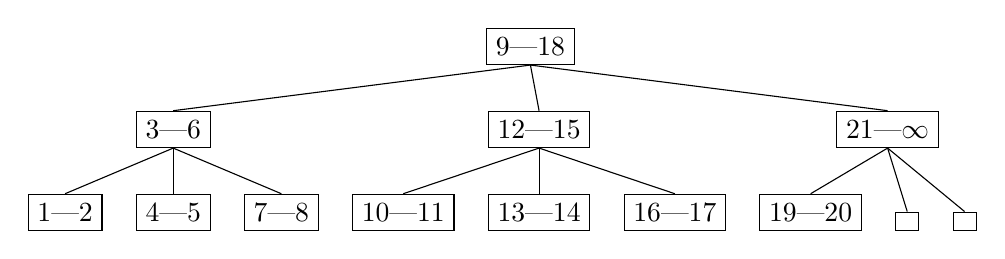
\begin{tikzpicture}[sibling distance=12pt]
    \tikzstyle{every node}=[rectangle,draw]
    \Tree [.9|18 [.3|6 1|2 4|5 7|8 ]  [.12|15 10|11 13|14 16|17 ] [.21|$\infty$ 19|20 $\,$ $\,$ ]]
  \end{tikzpicture}
\end{center}
The tree will be represented in a file in BFS layout:
$$9 \quad 18 \quad 3 \quad 6 \quad 12 \quad 15 \quad 21 \quad \infty \quad 1 \quad 2 \quad 4 \quad 5 \quad 7 \quad 8 \quad 10 \quad 11 \quad 13 \quad 14 \quad 16 \quad 17 \quad 19 \quad 20$$

\paragraph{Space and I/O complexity.} The construction algorithm copies the permutation of the $N$ keys from $A$ to a new file, and thus the total additional space needed in external memory is $O(N/B)$ blocks. After the preprocessing, $A$ is discarded, hence the auxiliary space is $O(1)$.

The I/O complexity of the step 3 in the first iteration is $O(N/B)$, because we move $m=N-N/(B+1)$ keys in $A \setminus L$, from $A$ to the new file, with $O(m/B)=O(N/B)$ read/write operations. Step 1 requires only $O(1)$ transfers to write the root block to the beginning of the new file. Steps 2 and 4 don't require any transfer from/to external memory, only CPU operations. Subsequent iterations of the algorithm work on smaller portions of $A$, thus the first iteration dominates with a total cost of $O(N/B)$ I/O operations.

  \section{Implicit navigation in vEB layout}
Consider $N = 2^h - 1$ keys where $h$ is a power of 2, and the implicit cache-oblivious vEB layout of their corresponding complete binary tree, where the keys are suitably permuted and stored in an array of length $N$ without using pointers (as it happens in the classical implicit binary heap but the rule here is different). The root is in the first position of the array. Find a rule that, given the position of the current node, it is possible to locate in the array the positions of its left and right children. Discuss how to apply this layout to obtain (a) a static binary search tree and (b) a heap data structure, discussing the cache complexity.

\vspace{0.5cm}
\paragraph{Solution.} We assume that the keys are stored in a zero-indexed array $A$ s.t. $\log A = H$. Given and index $0 \leq i < A.length$ we will give a rule for computing the index of its children.

\begin{center}
	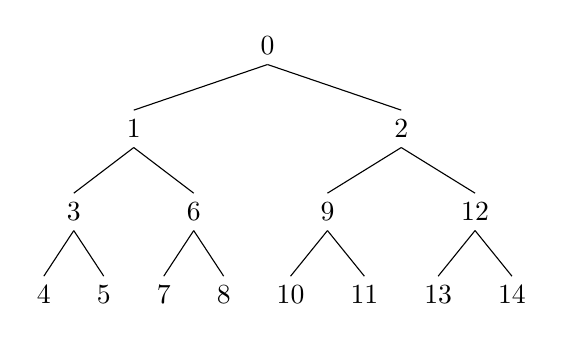
\begin{tikzpicture}[sibling distance=10pt]
	\Tree [.0 [.1 [.3 [.4 ]  [.5 ] ] [.6 [.7 ] [.8 ] ] ] [.2 [.9 [.10 ] [.11 ] ] [.12 [.13 ] [.14 ] ] ] ]
	\end{tikzpicture}
\end{center}

First, we define the \emph{cut distance} for a given node $v$.
Given that $T$ has height $h = 2^k$, each cut halves the current sub-tree $T', height(T') = 2{k'}$ producing sub-trees of height $\frac{2^{k'}}{2} = 2^{{k'} - 1}$.
Since the base case for the construction algorithm is $height(T') = 2$, this operation is repeated until a sub-tree of height $2$ is reached: therefore each node $v$ is at distance $d \leq 2$ from its next cut in the construction.
\subparagraph{Left and right children on $d(v) = 2$} By the above we have that on any even level (those for which $d(v) = 2$ holds) $l$ will have a left child $v' = v + 1$ and a right child in position $v'' = v + 2$.
As by construction the base case for $height(T') = 2$ is populated contiguously top-down left-to-right resulting in the above.
\subparagraph{Left and right children on $d(v) = 1$} By the above we have that on any even level (those for which $d(v) = 1$ holds) $l$ will have a left child $v' = v + \delta$ and a right child in position $v'' = v + \gamma$ for some $\delta, \gamma$.
The \emph{vEB} construction allocates space for each index crossing a path in a top-down left-to-right, as stated previously.
Now, since we are crossing a cut, we can either compute the size $\abs{T_{ls}}$ of all the $2LS$ sub-trees allocated before the left child and the size of the tree $T_{top}$ of height $l$ on top of $v$ and the size of the sub-trees on the left of our $v$.
\begin{equation} \label{15_top_size}
\abs{T_{top}} = 2^{l} - 1
\end{equation}
\begin{equation} \label{15_left_sub-trees_siblings}
\abs{T_{ls}} = \text{tree size } · \text{ number of trees }= 2^{H - l} \cdot 2LS
\end{equation}
with $2^{H - l}$ as size as we are at the $l$ level of a complete binary tree and $2LS$ siblings as the $LS$ nodes at level $l$ had two children each, again because we are in a complete binary tree.

Therefore our left child as children given by the size of the top tree $T_{top} + $ the size of its left siblings sub-trees $LSS$:
\begin{equation} \label{15_children}
\abs{T_{ls}} + \abs{T_{top}} = (2^{H - l})(2LS) + (2^{l+1} - 1)
\end{equation}

A search algorithm is then straightforward: starting from the root we traverse the node as a binary tree, keeping track of the variables needed by \ref{15_children}, namely level and left siblings (each increasing by 1 and by a factor of $2$ or $2 + 1$ respectively).

\paragraph{Binary search tree in vEB layout.} We now present a procedure to transform an array of keys $S$ to a tree $T$, stored in memory in vEB layout, that satisfies the binary search tree property (the key in each node must be greater than all keys stored in the left subtree, and not greater than all keys in the right subtree).
\begin{algorithmic}[1]
	\Require{$S$ sorted in ascending order}
	\Function{ArrayToVeb}{$S$, $i_{\text{vEB}}$, $l$, $r$}
	\If{$l > r$}
	\State \Return{}
	\EndIf
	\State $m \gets \lfloor (l+r)/2 \rfloor$
	\State $T[i_{\text{vEB}}] \gets S[m]$ \Comment{store the median in the root of the subtree}
	\State $l_{\text{vEB}} \gets $ \Call{Left}{$i_{\text{vEB}}$}
	\State $r_{\text{vEB}} \gets $ \Call{Right}{$i_{\text{vEB}}$}
	\State \Call{ArrayToVeb}{$S, l_{\text{vEB}}, l, m$}
	\State \Call{ArrayToVeb}{$S, r_{\text{vEB}}, m+1, r$}
	\EndFunction
\end{algorithmic}
The recursion starts from the call $\textsc{ArrayToVeb}(S, 0, 0, S.length-1)$. At the end of the procedure we can binary search in $T$ starting from the root $T[0]$, then traversing the implicit tree with the functions $\textsc{Left}$ and $\textsc{Right}$.

\begin{center}
	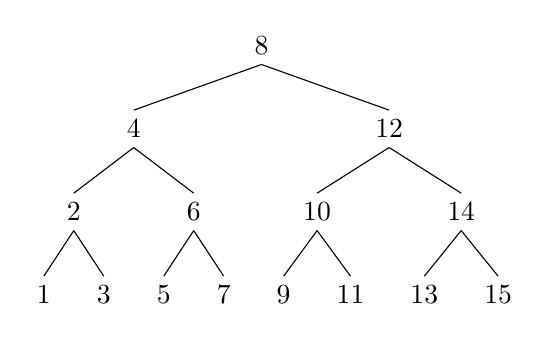
\begin{tikzpicture}[sibling distance=10pt]
	\Tree [.8 [.4 [.2 [.1 ]  [.3 ] ] [.6 [.5 ] [.7 ] ] ] [.12 [.10 [.9 ] [.11 ] ] [.14 [.13 ] [.15 ] ] ] ]
	\end{tikzpicture}
\end{center}

\paragraph{Heap tree in vEB layout.}  Given any array $S$ sorted in increasing (decreasing) order, the implicit tree with root $S[i]$, children $S[\textsc{Left}(i)]$ and $S[\textsc{Right}(i)]$, satisfies the min-heap (max-heap) property $\forall i \in [0, S.length-1]$.
  \section{1-D range query}
Describe how to efficiently perform one-dimensional range queries for the data structures described in Problems 14 and 15. Given two keys $k_1 \leq k_2$, a range query asks to report all the keys $k$ such that $k_1 \leq k \leq k_2$. Give an analysis of the cost of the proposed algorithm, asking yourself whether it is output-sensitive, namely, it takes $O(\log_B N + R/B)$ block transfers where $R$ is the number of reported keys.

\vspace{0.5cm}
\paragraph{Solution.}
  \section{External memory mergesort}
In the external-memory model (hereafter EM model), show how to implement the $k$-way merge (where $(k + 1)B \leq M$), namely, how to simultaneously merge $k$ sorted sequences of total length $N$, with an I/O cost of $O(N/B)$ where $B$ is the block transfer size. Also, try to minimize and analyze the CPU time cost.

\subsection{First solution}

We keep in main memory $k$ input buffers $B_1, B_2, \dots, B_k$ --- one for each sorted sequence $s_1, s_2, ..., s_k$ that we need to merge --- and 1 output buffer $B_{out}$. At each step we find the smallest unchosen element among the input buffers and copy this element to $B_{out}$. When $B_{out}$ is full, we write it to the end of a file $F$, then we clear $B_{out}$'s content.

For each input buffer we store a pointer $p_i$ to its first unchosen element. When a pointer $p_i$ reaches the end of the buffer $B_i$, we need to load in $B_i$ the next portion of the corresponding sorted sequence $s_i$ and reset $p_i$. We also store a pointer to the next free slot in $B_{out}$.

\paragraph{I/O complexity.} The $k$-way merge ends when we reach the end of every sorted sequence: we performed $\Theta(N/B)$ read operations for the sorted sequences, and $\Theta(N/B)$ writes to $F$, thus the total I/O complexity is $\Theta(N/B)$.

\paragraph{Minimizing CPU time.} The CPU complexity of searching the smallest element among the unchosen elements of the input buffers is $O(k)$. We can improve the algorithm by replacing the linear search with a minimum priority queue of the unchosen elements: in this way we can extract the smallest element in $O(1)$, advance the pointer $p_i$ of the corresponding input buffer $B_i$ and finally insert $B_i[p_i]$ in the priority queue in $O(\log k)$ time.

\subsection{Second solution}
Let
    \begin{itemize}
    \item $k = \frac{1}{4}\cdot \frac{M}{B}$ be the number of blocks the cache can hold.
    \item $B_s$ the blocks reserved in cache to store temporary merges.
    \item $N$ be the size of the problem.
    \item $B$ the block size, with $B_i$ a pointer to the $i^{th}$ block.
    \item $B_{i}^{c}$ the $i^{th}$ block stored in memory.
    \item $\frac{N}{B}$ the number of blocks storing $A$ in main memory.
    \end{itemize}
We assume the sorted blocks we receive in input are ordered and use $\frac{1}{3} \cdot \frac{M}{B}$ to store loaded blocks in a Fibonacci min-heap fashion.
\emph{k-way} mergesort operates on $k$ sorted blocks we load in cache.
We implement the merge operation as follows, outputting to external memory on file $O$:
    \begin{algorithmic}[1]
    \Function{merge}{$a$, $b$}:
    \For{$i \gets 0; i < k; i++$}
        \State load($B_i$, $B_i^m$)\;           \Comment{Load blocks in cache: $O(\frac{N}{B})$}
    \EndFor
    \State $busy\_blocks = k - 1$\;             \Comment{\parbox[t]{.5\linewidth}{Count busy blocks, that is blocks whose pointers have not reached
                                                        the end of the block}}
    \State $S \gets \&S$\;                      \Comment{\parbox[t]{.5\linewidth}{At most $O(k \cdot B)$, when every sorted block is greater than the following}}
    \While{$busy\_blocks > 0$}
        \State $m \gets \min\{\min{B_i^c}\}$\;  \Comment{Get the current minimum of every block in cache: $O(k)$}
        \State $B_j^c \gets B_j^c + 1$\;        \Comment{Shift to next element in block $B_j$ with current minimum element}
        \If{$B_j == EOB$}
            \State $busy\_blocks \gets busy\_blocks - 1$\;
        \EndIf
        \If{$busy\_blocks == 1$}
            \State $S \gets S :: flush(B_j^c)$\;    \Comment{Flush remaining block}
        \EndIf
        \State $*S \gets m$\;
        \State $S \gets S + 1$\;                \Comment{Increment storing blocks pointer}
    \EndWhile
    \State write(S, O)\;                        \Comment{Output}
    \EndFunction
\end{algorithmic}

As we assumed, our blocks are ordered Fibonacci min-heaps, thus allowing us to merge them in $k \cdot \log(n)$ time.
We can then store $S$ by finding the minimum element $n$ times in costant time: $n \cdot O(1) = O(n)$, giving us a total cost of
    \begin{equation*}
    k \cdot B + \log(k) \cdot O(k) + O(n)
    \end{equation*}
respectively for construction, find the minimum over $k$ Fibonacchi heaps in the \emph{merge} procedure and store it in memory.

  \section{External memory (EM) permuting}
Given two input arrays $A$ and $\pi^{-1}$, where $A$ contains $N$ elements and $\pi^{-1}$ contains a permutation of $\{1, \dots, N\}$, describe and analyse an optimal external-memory algorithm for producing an output array $C$ of $N$ elements such that $C[i] = A[\pi[i]]$ for $1 \leq i \leq N$.

\vspace{0.5cm}
\paragraph{Solution.}
\begin{enumerate}
	\item We define an array $\pi^{-1}$ such that $\pi^{-1}[i] = (\pi, i)$ of the form (departure, destination): note as we need $O(\frac{N}{B})$ block transfers.
	\item We then sort $\pi^{-1}$ according to the departure with the previously defined $k$-way mergesort in $O(\frac{N}{B} log_{\frac{M}{B}} \frac{N}{B})$ block transfers. $\pi^{-1}$ now holds the ordered departures with respective index where to send the elements to (the destination).
	\item We can now build $A\pi^{-1}$ with entries $(\pi^{-1}[i].destination, A[i])$ of the form (destination, element).
	As we ordered by the departures we scan $A$ sequentially: $A\pi^{-1} = [(destination, A[0]),$ \\$(destination, A[1]), (destination, A[2]), \dots]$: again we have $O(\frac{N}{B})$ block transfers.
	\item We run one more ordering over such tuples in $A\pi^{-1}$, this time according to the destination: we now have an ordered mapping \emph{destination}($\pi[i]$) $\to$ \emph{element} and we are able to write it to memory with $O(\frac{N}{B})$ block transfers:
	\begin{gather*}
	  sort(A\pi^{1}) = [(0, A[x]), (1, A[x]), (2, A[y]), (3, A[x]), \dots ] = \\
	  = [(0, A[\pi[0]]), (1, A[\pi[1]]), (2, A[\pi[2]]), (3, A[\pi[3]]), \dots ] 
	\end{gather*}
\end{enumerate}
The I/O complexity of the solution is dominated by the cost of sorting, that is $O(\frac{N}{B} log_{\frac{M}{B}} \frac{N}{B})$.
  \section{Suffix sorting in EM}
Using the DC3 algorithm seen in class, and based on a variation of mergesort, design an EM algorithm to build the suffix array for a text of $N$ symbols.
The I/O complexity should be the same as that of standard sorting, namely, $O(\frac{N}{B} log_{\frac{M}{B}} \frac{N}{B})$ block transfers.

\vspace{0.5cm}
\paragraph{Solution .}
We improve the \emph{DC3} algorithm by exploiting the multi-way mergesort defined in exercise 17.
To give a proper overview we'll insert the complete algorithm, highlighting the differences introduced.

\subparagraph{Samples construction}
We split our string $A$ of size $3N$ in two chunks $S_0, S_1, S_2$ each of size $N$ according to the index of each character: $c \in S_i \iff i \mod 3 = i$.
We are able to do so in linear $O(N)$ time and $\frac{N}{B}$ cache loads, as a linear scan is sufficient.

\subparagraph{Sample sorting}
We now twitch a little bit the \emph{DC3}: instead of operating a traditional radix-sort in order to sort $S_{1,2}$ we apply our multi-way merge-sort on $k = \frac{M}{B}$ \emph{3-grams}, ordering them in $\frac{M}{B} \log_k(\frac{M}{B})$.
The use of multi-way merge-sort allows us to reduce computation time and cache cost, thus allowing us to stay in the boundary of $O(\frac{N}{B} log_{\frac{M}{B}} \frac{N}{B})$.
Storage of $S^-1[A]$ still takes linear time and $\frac{M}{B} + \frac{1}{3} \cdot \frac{M}{B}$ cache writes, as $\frac{1}{3} \cdot \frac{M}{B}$ single values (the ranks) need to be stored.

\subparagraph{Non-sample sorting}
As operations over $S_0$ are trivial lexicographic comparisons, we are able to load them in $\frac{3N}{B}$ cache loads and sort them using again our multi-way merge-sort obtaining the above results.
We can further improve by then writing the merge 3-tuples of $S_{0,1}, S_{0,2}, S_{1,2}$ to disk in linear time: as they are constructed with $\frac{M}{B}$ cache loads for $S_{1,2}$, $\frac{M}{B}$ cache loads for $S_{0}$ and $\frac{M}{B}$ cache loads for their respective ranks.

\subparagraph{Merging}
We then merge the ranks computed in the sample and non-sample sorting of step 2 and 3 of the algorithm with the multi-way merge-sort whose comparison operator is the same used by the classical \emph{DC3} algorithm.
  \section{Wrong greedy for minimum vertex cover}

Find an example of (family of) graphs for which the following greedy approach fails to give a 2-approximation for the minimum vertex cover problem (and prove why this is so). 
Start out with an empty $\tilde{S}$.
Choose each time a vertex $v$ with the largest number of incident edges in the current graph.
Add $v$ to $\tilde{S}$ and remove its incident edges.
Repeat the process on the resulting graph as long as there are edges in it.
Return $\abs{\tilde{S}}$ as the a approximation of the minimal size of a vertex cover for the original input graph.
Generalize your argument to show that the above greedy algorithm cannot actually provide an $r$-approximation for any given constant $r >1$.

\paragraph{Solution}
We create a class of graphs $G = (V, E), \abs{V} = N$ s.t. $V$ is partitioned in $S, R$ s.t. $\abs{S} = k, \abs{R} = \sum_{i = 1}^{k} \left(\lfloor{\frac{k}{i}} \rfloor \right)$ respectively and define them as \emph{senders} and \emph{receivers}.

We then build the edges in the following way in order to obtain a minimum cover $L$:
	\begin{enumerate}
	\item For the current iteration $i$, if $\lfloor{\frac{k}{i}}\rfloor = 0$ we stop.
	\item Split the current slice $R$, consider the first $\lfloor{\frac{k}{i}}\rfloor$ vertexes: let $R^i$ be this slice.
	\item For every vertex $v \in R^i$ build $\frac{m}{\lfloor{\frac{k}{i}}\rfloor}$ outgoing edges to each of the $m$ nodes $\in R$.
	We can then repeat step $1$ with $R \gets R \setminus R^i$.
	\end{enumerate}
Once the above procedure ends, we have partitions vertexes of size $k \in S: deg(v) = 1$, one partition of vertexes of size $\lfloor{\frac{k}{2}}\rfloor \in S: deg(v) = \lfloor{\frac{k}{2}}\rfloor \forall v \in S$, etc. 
Each node in $R$ will have an incoming edge for every node $n \in L$ and will therefore be in the minimum vertex cover, as by hypothesis $\abs{S} > \abs{R}$
The greedy algorithm then starts by removing the highest-degree node: we find this on top of $R$, as it was doubled at each iteration.
By construction we have $k$ \emph{senders} partitions whose highest degree is $k$ (note as the degree increases in the summation up to $\lfloor{\frac{k}{i}}\rfloor$ for $i = k$).
The \emph{receivers} have a maximum degree of $\sum_{i = 1}^{k} \lfloor{\frac{k}{i}}\rfloor \approx k \ln k$,
as each of them received an incoming edge from each partitions $\in S$ that we asserted being $\lfloor{\frac{k}{i}}\rfloor$ by construction.
The greedy algorithm will start removing from the vertex with highest degree: it will be forced to remove from the last built slices up to $\lfloor{\frac{k}{i}}\rfloor > \frac{m}{\lfloor{\frac{k}{i}}\rfloor}$, thus cutting at least $k \ln k > m$ vertexes before cutting in the minimum cover $S$.
We can build a family of such graphs by making $k$ grow at will: as $k \ln k > r \forall k$ such family will have an increasingly larger \emph{r-approximation}:
\begin{equation*}
  k \ln k > rk \text{ }\forall k, r
\end{equation*}
  \section{Greedy  2-approximation for  MAX-CUT  on  weighted  graphs}
Prove  that  the  greedy algorithm for \emph{MAX-CUT} described in class gives also a $2$-approximation for weighted graphs with positive weights.

\paragraph{Solution.}
Let $G$ be our undirected weighted graph with $n$ nodes and $m$ edges.
As stated in class, the greedy algorithm scans sequentially the ordered nodes, deciding at each iteration $i$ whether to add the node $v$ to the cut or not by computing the following:
	\begin{algorithmic}[1]
	\Function{add?}{$v$, $S$}
	\State $S' \gets S \cup \{v\}$\;
	\If{$E(S') > E(S)$}
		\State $S \gets S'$\;
	\EndIf
	\EndFunction
	\end{algorithmic}
With a weighted graph we need to slightly modify the above:
	\begin{algorithmic}[1]
	\Function{add?}{$v$, $S$}
	\State $S' \gets S \cup \{v\}$\;
	\If{$\sum_{n \in S'}{w(n)} > \sum_{n \in S}{w(n)}$}
	\State $S \gets S'$\;
	\EndIf
	\EndFunction
\end{algorithmic}
The above is computed for each vertex $v$ in local search but only $r_v = \abs{E_v}, E_v = \{v' | \exists e(v + \delta, v) \in E\}$ for the greedy algorithm, that is the nodes with a greater ordering and with a colliding edge on $v$.
By applying the above function we have an $r'_v$.
We also know that in a non-weighted case, given any vertex $u$, at least $\frac{r_u}{2}$ vertexes are in the cut: if this was not true, then we could add one cut, switching $v$ from $S$ to $\bar{S}$ or vice versa increasing the number of nodes in the cut.
A weighted variant is trivial: as the non-weighted case chooses to switch $v$ according to $\sum{r^i}$, we choose to switch according to the weight sum $\mathcal{W} = \sum{\omega(r^i)}$.
It follows that $r'_v = \sum{\omega(\text{edges incident to v in the cut}}) \geq \sum{\frac{\omega \left( \text{incident edges on v} \right)}{2}}$. \\
Therefore we have the weights in the cut
\begin{equation}
E_{\omega} = \sum_{v \in V}{\frac{\omega(r'_v)}{2}} =
\frac{1}{2} \sum_{v \in V}{\omega(r'_v)} =
\frac{1}{2} \mathcal{W(G)}
\end{equation}
  \section{Randomized 2-approximation for MAX-CUT}

Prove  that  the  following  randomized algorithm provides a $2$-approximation for MAX-CUT in expectation, namely, the expected cut size is at least half of the optimal cut size.
Here are the steps.
\emph{(1)} For each vertex $v \in V$,  toss  an  unbiased  coin:  if  it  is  tail, insert $v$ into $C$; else, insert $v$ into $V \setminus C$.
\emph{(2)} Start out with an empty set $T$.
For each edge $\{v, w\} \in E$, such that $v \in C$ and $w \in V \setminus C$, add $\{v, w\}$ to $T$.
Return $\abs{T}$ as approximated solution.

\vspace{0.5cm}
\paragraph{Solution.}
We define the indicator variable $X_{v, w}$ in order to establish whether $e\{v, w\} \in T$:
\begin{equation*}
X_{v, w} =   \begin{cases}
1   & \text{if } \{v, w\} \in T \\
0   & \text{otherwise}
\end{cases}
\end{equation*}
with 
\begin{gather*}
\Pr(X_{v, w} = 1) = \Pr(v \text{ colored }, w \text{ not colored } \lor v \text{ not colored }, w \text{ colored }) = \\
\Pr(v \in C, w \notin C \lor v \notin C, w \in C) =
\frac{1}{4} + \frac{1}{4} = \frac{1}{2}
\end{gather*}
and expected value $\E{X_{v,w}} = \frac{1}{2} \cdot 1 + \frac{1}{2} \cdot 0 = \frac{1}{2}$.

We then define the indicator variable $X$ for all the cuts we might have:
\begin{equation*}
X = \sum_{(v, w) \in E} X_{v, w}
\end{equation*}
with expected value $\E{X}$:
\begin{equation*}
\E{X} = \E{\sum_{(v, w) \in E} X_{v, w}} = \sum_{(v, w) \in E} \E{X_{v, w}} = \frac{1}{2} \abs{E}
\end{equation*}
The cut we obtain through the above algorithm:
\begin{equation*}
\E{X} = \frac{1}{2} \abs{E}
\end{equation*}
Given $\abs{OPT} \leq \abs{E}$ optimal cut we have an approximated solution $r$ of:
\begin{equation*}
r = \frac{\abs{OPT}}{\E{X}} \leq \frac{\abs{E}}{\frac{1}{2}\abs{E}} = 2 
\end{equation*}
  \appendix
\section{Hogwarts}

The Hogwarts School\footnote{\url{http://didawiki.cli.di.unipi.it/lib/exe/fetch.php/magistraleinformatica/alg2/algo2_16/hogwarts.pdf}}
is modeled as a graph $G=(V, E)$ where $V$ is the set of castle's rooms and $E \subseteq V \times V$
is the set of the stairs.
Each stair is labelled with the time of appearance and disappearance, and can be
walked in both directions, therefore the graph is undirected.
The goal is to find, if possible, the minimum amount of time required to go from
the first to the last room.

\subsection{Solution 1: Preprocessing-then-Dijkstra}

Dijkstra is able to find the shortest path in a graph with non-negative weights
on its edges.
Our main idea is to create a Dijkstra compatible graph through a \textsc{normalize}
function, then apply Dijkstra to it in order to find the shortest path.
The core of the preprocessing is the \textsc{normalize} function which computes traversal
times between nodes at a given time \emph{time}:

\begin{algorithmic}[1]
  \Function{normalize}{$from$, $to$, $time$}:
    \State $t \gets \infty$
    \If{$start[v'] \leq t < end[v']$}  \Comment{No waiting time}
      \State $t \gets t + 1$
    \ElsIf{$t < start[v']$}            \Comment{Waiting time}
      \State $t \gets start[v'] + 1$
    \Else
      \State $t \gets \infty$          \Comment{Available time already expired}
    \EndIf
      \State \Return{$t$}
    \EndFunction
\end{algorithmic}

The normalize function is then applied to a node traversal:

\subsubsection{Pseudo-code}

\begin{algorithmic}[1]
  \State create vertex set $Q$ of unvisited nodes\;
  \State create vertexes set $E'$ of edges weight\;
  \State $time \gets 0$                   \Comment{Initial time for traversal}
  \State $edges \gets$ \Call{stairs\_of}{0}\;      \Comment{Get incoming/outgoing edges
   of the source node}
  \Function{process}{$node$, $time$}
    \If{$edge \in visited\_edges$}
      \State \Return{}
    \EndIf

    \State $traversal\_time \gets \infty$
    \ForAll{$neighbor \in neighbors\_of\_node$}
      \State $traversal\_time \gets$ \Call{traversal\_time}{$node$, $neighbor$, $time$}
      \State $E'[0][node] \gets traversal\_time$   \Comment{$E'[i][j]$ holds the
                                                        weight/traversal}
      \State \Comment{time for the stair between $i$ and $j$}

      \ForAll{$new\_neighbor \in neighbors\_of\_neighbor$}
        \State \Call{normalize}{$neighbor$, $new\_neighbor$, $traversal\_time$}
      \EndFor
    \EndFor
    \If{\Call{dijkstra}{$V, E'$} = $\infty$}
    	\State \Return{-1}
    \Else
      \State \Return{$t$}
    \EndIf
  \EndFunction
\end{algorithmic}

\begin{framed}
  \noindent
  \textbf{Computational cost}: $\Theta(n^{2})$ if the vertex set in \textsc{dijkstra} is implemented
  as an array. $O(|E|+|V|\log |V|)$ with Fibonacci heap.
\end{framed}

\subsection{Solution 2: HogwartsDijkstra}

\begin{algorithmic}[1]
  \Function{HogwartsDijkstra}{$G$}:
  \State create vertex set $Q$ of unvisited nodes
  \ForAll{vertex $v \in V$}      \Comment{initialization}
      \State $time[v] \gets \infty$  \Comment{unknown time from source to v}
      \State add $v$ to $Q$          \Comment{all nodes initially in Q}
  \EndFor
  \State $time[0] \gets 0$ \Comment{time from source to source}
  \While{$Q\ne \emptyset$}
      \State $u \gets x \in Q$ with $\min \{time[x]\}$
      \State remove $u$ from $Q$
      \ForAll{neighbor $v$ of $u$}:
          \If{$time[u] \leq appear[v]$}
              \State $alt \gets appear[v] + 1$ \Comment{wait the appearance of
                                                                    the stair}
          \ElsIf{$time[u] < disappear[v]$}
              \State $alt \gets time[u] + 1$       \Comment{use the stair}
          \Else
              \State $alt \gets \infty$            \Comment{the stair has
                                                        already disappeared}
          \EndIf
          \If{$alt < time[v]$}
              \State $time[v] \gets alt$           \Comment{a quicker path to
                                                            $v$ has been found}
          \EndIf
      \EndFor
  \EndWhile
  \State \Return{$time[|N|-1]$}
  \EndFunction
\end{algorithmic}

\begin{framed}
  \noindent
  \textbf{Computational cost}. See the previous section.
\end{framed}

\subsection{Solution 3: BFS-like traversal}

\begin{algorithmic}[1]
  \Function{reach}{$N$, $M$, $A[]$, $B[]$, $appear[]$, $disappear[]$}
      \For{$i=0$ to $M-1$}
          \State $edges\_[A[i]].push\_back(make\_pair(i, B[i]))$
          \State $edges\_[B[i]].push\_back(make\_pair(i, A[i]))$
      \EndFor
      \For{$i=0$ to $N-1$}
          \State $done\_[i] \gets false$
          \State $distance\_[i] \gets \infty$
      \EndFor
      \State $reached\_[0].push\_back(0)$
    \State $distance\_[0] \gets 0$
    \For{$t=0$ to $MAX\_TIME$}
      \ForAll{$v \in reached\_[t]$}
          \If{not $done\_[v]$}
          \ForAll{$edge \in edges\_[v]$}
            \State $staircase \gets edge.first$
            \State $neighbor \gets edge.second$
            \State $time \gets \max(distance_[v], appear[staircase])+1$
            \If{not $done\_[neighbor]$ \\ \hfill and $distance\_[v] < disappear[staircase]$ \\ \hfill and  $time < distance\_[neighbor]$}
              \State $distance\_[neighbor] \gets time$
              \State $reached\_[time].push\_back(neighbor)$
            \EndIf
          \EndFor
        \State $done\_[v] \gets true$
          \EndIf
      \EndFor
    \EndFor
    \State \Return{$(distance\_[N-1] = \infty) ? -1 : distance\_[N-1]$}
  \EndFunction
\end{algorithmic}

\begin{framed}
  \noindent
  \textbf{Computational cost}: $O(m + MAX\_TIME)$.
\end{framed}


\section{Paletta}

Paletta ordering\footnote{\url{http://didawiki.cli.di.unipi.it/lib/exe/fetch.php/magistraleinformatica/alg2/algo2_16/paletta.pdf}}
is a peculiar ordering technique: given a 3-tuple of elements, paletta takes the
central element as pivot and swaps the two elements right before and next to it.
To make an example:
$$(3, 2, 1) \xrightarrow{paletta} (1, 2, 3)$$
We now want to develop an algorithm to order any array through paletta ordering
with the minimal number of swaps.
You should see as not every array can be ordered (e.g. [1, 3, 2]).

\vspace{0.5cm}
\paragraph{Solution.}
We should note that the following properties hold:
\begin{enumerate}
    \item Every element can be a pivot, but the first and the last one, as they
    have respectively no elements before and after them.
    \item Every element can be swapped as many times as necessary, but only with
    elements of the same 2-remainder (numbers in even positions can only be
    swapped with numbers in even positions, the same holds for odd indexes).
    More formally, if $n$ is the size of the array $A$ we want to sort,
    $i,j \in [1, n - 2]$, $A[i]$ can be swapped with $A[j]$ if and only if $i \equiv j \pmod{2}$.
    \item The least number of swaps does not backtrack any element.
    Formally, let \emph{k} be the minimal number of swaps applied to an array,
    backtracks included. By hypothesis, \emph{k} is minimal, but at least \emph{m},
    $m > 0$ backtrack swaps have been operated, therefore we found a
    $k' = k - m: k' < k$, a new minimal number of swaps: contradiction.
\end{enumerate}

Given item 2, we can split our array in two, even and odd numbers, and order
them counting the swaps.
In our example we'll use \emph{mergesort}, as it runs in $O(n\log n)$, does
backtrack elements, and is very well-known.
Clearly, given an array, a swap happens when an element is pushed back, pulling
the one between its new position and the old one ahead: we can map this behaviour
in the merge routine of mergesort: the array merged is able to push back elements
from its right pointer to the new array, moving them back of $(m - i) + (j - m)$ positions,
where \emph{m} is the dimension of the current two sub-arrays to merge.
Provided that our edited version of mergesort ran successfully on both the
even-index and odd-index, we now need to verify if by merging them we obtain an
ordered array.
Intuitively, the merged array will start with the first element of the even-index
arrays, followed by the first of the odd-index array, followed by the second of
the even-index array, and so on.
To check for these elements is pretty trivial and can be done in linear time.
Follows the pseudo-code for the edited version and \textsc{snake\_check} function:

\begin{algorithmic}[1]
  \Function{merge\_with\_paletta}{$left$, $right$, $k$}:
    \State \dots                        \Comment{merge instructions}
    \If{$right > left$}
      \State $paletta\_count \gets paletta\_count + 1$
      \State \dots
      \EndIf
    \EndFunction
\end{algorithmic}

\begin{algorithmic}[1]
  \Function{snake\_check}{}
    \State $even, odd \gets 0$
    \For{;$even, odd < N;even = even + 1, odd = odd + 1$}
      \If{$a[even] > a[odd]$}
        \State \Return{$-1$}\;
      \EndIf
    \EndFor
    \State \Return{$paletta\_count$}\;
    \EndFunction
\end{algorithmic}

\begin{framed}
  \noindent
  \textbf{Computational cost}: $\Theta(n\log n)$.
\end{framed}


  \printbibliography

\end{document}
